\chapter{Results}

\section{Resnet}

\subsection{Linear evaluation on features}


The following Figure~\ref{fig:spider_resnet50} shows the result with Resnet50, while Table~\ref{tab:f1_scores_resnet_derma} and Table~\ref{tab:f1_scores_resnet_plant} contain the respective values.
\begin{figure}[H]
    \begin{center}
    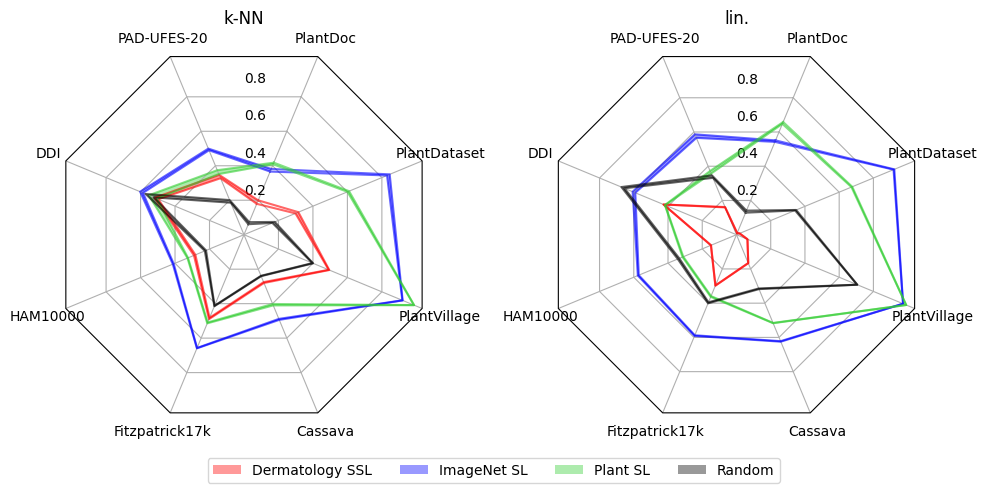
\includegraphics[width=15cm]{../images/spider_resnet50.png}
    \caption{Linear evaluation of Resnet50}\label{fig:spider_resnet50}
    \end{center}
\end{figure}

The first thing to notice is the really bad performance of the model trained on dermatology with SimCLR. The scores are never significantly better than the other pre-trained models. The model which was trained on ImageNet with \gls{ssl} was not put into the graphic but the tables show that these scores are bad as well. 
This indicates a problem with the type of training rather than with the data per se.

In the linear evaluation the plant based model is actually a little bit better than the ImageNet based model, but with \gls{knn} the difference becomes negligible.

\begin{table}[H]
\centering
\caption{F1-scores of ResNet50 on dermatology downstream tasks\label{tab:f1_scores_resnet_derma}}
{\fontsize{8pt}{10pt}\selectfont 
\csvreader[tabular=|l|c|c|c|c|c|c|c|c|,
filter expr={test{\ifnumgreater{\thecsvinputline}{3}}},
table head=\hline\multicolumn{1}{|c|}{} & \multicolumn{2}{c|}{\bfseries DDI} & \multicolumn{2}{c|}{\bfseries PAD-UFES-20} & \multicolumn{2}{c|}{\bfseries HAM10000} & \multicolumn{2}{c|}{\bfseries Fitzpatrick17k}\\\hline Pre-training & Lin. & k-NN & Lin. & k-NN & Lin. & k-NN & Lin. & k-NN \\\hline,
table foot=\hline]{../results/f1_scores_resnet_derma.csv}{}%
{\csvcoli\ & \csvcolii & \csvcoliii & \csvcoliv & \csvcolv & \csvcolvi & \csvcolvii & \csvcolviii & \csvcolix}%
}
\end{table}

\begin{table}[H]
\centering
\caption{F1-scores of ResNet50 on plant downstream tasks\label{tab:f1_scores_resnet_plant}}
{\fontsize{8pt}{10pt}\selectfont 
\csvreader[tabular=|l|c|c|c|c|c|c|c|c|,
filter expr={test{\ifnumgreater{\thecsvinputline}{3}}},
table head=\hline\multicolumn{1}{|c|}{} & \multicolumn{2}{c|}{\bfseries PlantDoc} & \multicolumn{2}{c|}{\bfseries PlantDataset} & \multicolumn{2}{c|}{\bfseries Cassava} & \multicolumn{2}{c|}{\bfseries PlantVillage}\\\hline Pre-training & Lin. & k-NN & Lin. & k-NN & Lin. & k-NN & Lin. & k-NN \\\hline,
table foot=\hline]{../results/f1_scores_resnet_plant.csv}{}%
{\csvcoli\ & \csvcolii & \csvcoliii & \csvcoliv & \csvcolv & \csvcolvi & \csvcolvii & \csvcolviii & \csvcolix}%
}
\end{table}

\section{Vision Transformers}

The results of the \gls{vit} can bee seen in Figure~\ref{fig:spider_vit}, Table~\ref{tab:f1_scores_vit_derma} and Table~\ref{tab:f1_scores_vit_plant}. 
The scores look similar. The scores of the plant based model are better in some tasks than the model trained with \gls{sl} on ImageNet, but not better than der \gls{ssl} variant. All DINO based models are relatively close to each other. This is probably due to their way of training rather than the data.

\begin{figure}[H]
    \begin{center}
    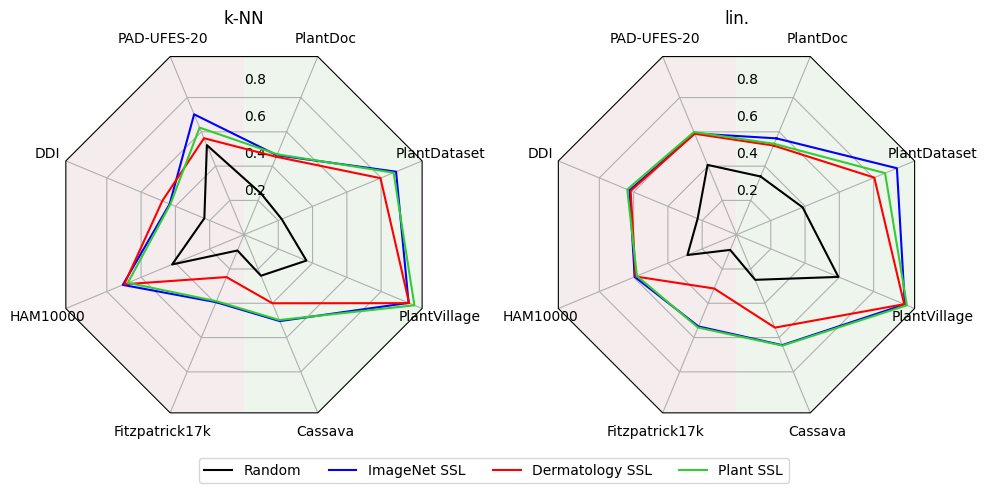
\includegraphics[width=15cm]{../images/spider_vit.png}
    \caption{Linear evaluation of \gls{vit}}\label{fig:spider_vit}
    \end{center}
\end{figure}


\begin{table}[H]
\centering
\caption{F1-scores of ViT-T16 on dermatology downstream tasks\label{tab:f1_scores_vit_derma}}
{\fontsize{8pt}{10pt}\selectfont 
\csvreader[tabular=|l|c|c|c|c|c|c|c|c|,
filter expr={test{\ifnumgreater{\thecsvinputline}{3}}},
table head=\hline\multicolumn{1}{|c|}{} & \multicolumn{2}{c|}{\bfseries DDI} & \multicolumn{2}{c|}{\bfseries PAD-UFES-20} & \multicolumn{2}{c|}{\bfseries HAM10000} & \multicolumn{2}{c|}{\bfseries Fitzpatrick17k}\\\hline Pre-training & Lin. & k-NN & Lin. & k-NN & Lin. & k-NN & Lin. & k-NN \\\hline,
table foot=\hline]{../results/f1_scores_vit_derma.csv}{}%
{\csvcoli\ & \csvcolii & \csvcoliii & \csvcoliv & \csvcolv & \csvcolvi & \csvcolvii & \csvcolviii & \csvcolix}%
}
\end{table}

\begin{table}[H]
\centering
\caption{F1-scores of ViT-T16 on plant downstream tasks\label{tab:f1_scores_vit_plant}}
{\fontsize{8pt}{10pt}\selectfont 
\csvreader[tabular=|l|c|c|c|c|c|c|c|c|,
filter expr={test{\ifnumgreater{\thecsvinputline}{3}}},
table head=\hline\multicolumn{1}{|c|}{} & \multicolumn{2}{c|}{\bfseries PlantDoc} & \multicolumn{2}{c|}{\bfseries PlantDataset} & \multicolumn{2}{c|}{\bfseries Cassava} & \multicolumn{2}{c|}{\bfseries PlantVillage}\\\hline Pre-training & Lin. & k-NN & Lin. & k-NN & Lin. & k-NN & Lin. & k-NN \\\hline,
table foot=\hline]{../results/f1_scores_vit_plant.csv}{}%
{\csvcoli\ & \csvcolii & \csvcoliii & \csvcoliv & \csvcolv & \csvcolvi & \csvcolvii & \csvcolviii & \csvcolix}%
}
\end{table}


% \subsection{Subsampling}

% \section{Other}
% \subsection{DINO student/teacher}
% \subsection{Fine-tuning}
% \subsection{Fine-tuning}
